\documentclass{article}

\usepackage[utf8]{inputenc}   %for german letters ä,ö...
\usepackage[ngerman]{babel}   %german settings
\usepackage{amsmath}
\usepackage{amssymb}
\usepackage{tikz,pgfplots}
\usetikzlibrary{patterns}
\usepackage[justification=centering]{caption}
\usepackage[left=3cm,right=3cm,top=2cm,bottom=3cm]{geometry}
\usepackage[tight-spacing=true]{siunitx}
\usepackage{booktabs}
\usepackage[outdir=./]{epstopdf}
\usepackage{subcaption}
\usepackage{placeins}
\usepackage{esdiff}

\usepackage{mathrsfs}
\usetikzlibrary{arrows}
\newcommand{\degre}{\ensuremath{^\circ}}

\usetikzlibrary{patterns}
\tikzstyle{spring}=[thick,decorate,decoration={zigzag,pre length=0.3cm,post length=0.3cm,segment length=6}]

\sisetup{locale = DE}

\newcommand{\upd}[1]{^\mathrm{#1}}
\newcommand{\ind}[1]{_\mathrm{#1}}
\newcommand{\RM}[1]{\MakeUppercase{\romannumeral #1}}


\usepackage[backend=bibtex8,sorting=none]{biblatex}
\addbibresource{refs.bib}

\begin{document}
\setlength{\parindent}{0em}   %Einrücken verhindern
\title{Physikalisches Praktikum \RM{4}\\Versuch 401\\Elektronische Übergänge in Atomen}
\author{Kilian Bönisch \ \ \ \qquad s6kiboen@uni-bonn.de \qquad 2897138\\
  Friedrich Hübner \qquad s6frhueb@uni-bonn.de \qquad 2897111}
\date{27.11.17}

\maketitle

\newpage

\thispagestyle{empty}

\tableofcontents

\newpage

\section{Einleitung}
In diesem Versuch wird das Verhalten von Spin-$\frac{1}{2}$-Teilchen in einem äußeren Magnetfeld untersucht. Dafür wird eine Probe mit Mineralöl in dem Magnetfeld platziert und die Dynamik des Spins der Protonen beobachtet. Charakteristische Zeitkonstanten die mit der Spin-Spin und Spin-Gitter Wechselwirkung zusammenhängen werden bestimmt.


\section{Zeeman-Effekt}
\subsection{Theoretische Vorbetrachtungen}
\subsubsection{Spektrallinien}
Die Energie-Eigenzustände des Wasserstoffatoms werden durch die Quantenzahlen $n,l$ und $m$ beschrieben. Ein Zustand mit der Hauptquantenzahl $n$ hat dabei den Energie-Eigenwert $E_n=-R\ind{y}/n^2$, wobei $R\ind{y} = hc\cdot \cfrac{R_\infty}{1+\frac{m\ind{e}}{m\ind{K}}}$ die Rydberg-Energie ist ($m\ind{K}$ Kernmasse). Wechselt das Wasserstoffatom von einem Zustand mit Hauptquantenzahl $n$ zu einem energetisch niedrigeren Zustand mit Hauptquantenzahl $n'$ wird ein Photon der Energie 
\begin{align*}
  E_{n \rightarrow n'}&=R\ind{y} \left( \frac{1}{n'^2} - \frac{1}{n^2}\right)
\end{align*}
emittiert. Die Balmer-Serie enthält alle Frequenzen des Emissionsspektrums, die aus dem Übergang von einem Niveau $n>2$ auf das Niveau $n'=2$ entstehen. Daraus ergibt sich folgender Zusammenhang für die Wellenlängen:
\begin{align}
  \cfrac{1}{\lambda} = \cfrac{R_\infty}{1+\frac{m\ind{e}}{m\ind{K}}} \left( \frac{1}{2^2} - \frac{1}{n^2}\right)
  \label{equ:rydberg}
\end{align}

Daran kann man auch die Isotopieaufspaltung erkennen: Für unterschiedliche Kernmassen $m\ind{K}$ ergeben sich leicht unterschiedliche Wellenlängen. 

\subsubsection{Linienbreite}
In der Praxis haben die beobachtbaren Balmer-Linien eine gewisse Ausdehnung. Mögliche Ursachen dafür sind:
\begin{itemize}
\item    
Durch die thermische Bewegung der Atome kommt es zur Dopplerverschiebung der Wellenlänge des emittierten Lichtes. Bewegt sich das Atom mit der Geschwindigkeit $v$ auf den Empfänger zu und emittiert ein Photon der Wellenlänge $\lambda$, so misst dieser die Wellenlänge 
\begin{align*}
  \lambda'=\lambda \cdot \left(  1+ \frac{v}{c} \right),
\end{align*} 
wobei $c$ die Lichtgeschwindigkeit ist. Nimmt man an, dass es sich bei dem Gas der Gasentladungsröhre um ein ideales Gas handelt, gilt für die Geschwindigkeit $v$ jedes Atoms (mit Masse $m$ und Boltzmann-Konstante $k_\mathrm{B}$)
\begin{align*}
  \frac{1}{2} m\ind{K} v^2=\frac{3}{2} k_\mathrm{B} T.
\end{align*}
Durch die Dopplerverschiebung schwankt die Wellenlänge also im Bereich
\begin{align}
  \sigma[\lambda]\ind{Doppler}=\frac{\lambda}{c}\sqrt{\frac{3k\ind{B}T}{m\ind{K}}}.
  \label{equ:doppler}
\end{align}
\item Es gibt eine natürliche Linienbreite. Nach \cite{unschaerfe} gilt, dass wenn ein angeregter Zustand des Atoms die mittlere Lebensdauer $\tau$ hat, die Spektrallinie dieses Zustandes die Form einer Lorentz-Kurve mit Breite 
\begin{align}
  \sigma[E]\ind{n}&=\frac{\hbar}{\tau}\nonumber\\
  \sigma[\lambda]\ind{n} &= \frac{\lambda^2}{2\pi c \tau}
  \label{equ:natbreite}
\end{align}
hat.
\end{itemize}

\subsection{Winkelverteilung}

Im ersten Versuchsteil wird die Winkelverteilung der Höhenstrahlung gemessen. Dazu werden 24 Detektoren (Z1-Z24) kreisförmig angeordnet und ein zusätzlicher Detektor (Z25) in die Mitte des Kreises gestellt (siehe Abb. \ref{fig:winkel_skizze}). Jeder Detektor ist mit einem Diskriminator verbunden, der ab einer bestimmten Schwelle einen Puls abgibt (Längen der Pulse: Oben: 30ns, Unten: 50ns, Z25: 100ns).
Geben gleichzeitig drei Detektoren, die auf einer Linie liegen ein Signal, so wird diese Koinzidenz als Teilchendurchgang identifiziert. Man zählt nun über einen bestimmten Zeitraum die Anzahl der Koinzidenzen aus allen Richtungen und erhält somit die Verteilung der Höhenstrahlung.

\begin{figure}[h]
\centering
\includegraphics[scale=0.9]{img/winkel_skizze.png}
\caption{Anordnung der Detektoren\cite{praktikumsheft}}
\label{fig:winkel_skizze}
\end{figure}

\subsubsection{Schwellenkurve}
Bevor man die Winkelverteilung messen kann, muss zuerst die optimale Schwelle für den Diskriminator D12 bestimmt werden. Die Schwellen der anderen Diskrimatoren sind schon eingestellt. Dazu wird die Schwelle des Diskrimators von -50 bis -250 \si{\milli\volt} in 10 \si{\milli\volt} Schritten verändert und jeweils für 2520 \si{\second} die Anzahl der Koinzidenzen von D12 mit D23, D24, D1 oder D2 gemessen. Dies wird über ein LabVIEW-Programm automatisiert (siehe Abb. \ref{fig:prog_all}).\\

Im ersten Teil des Programmes wird die Hardware initialisiert (siehe Abb. \ref{fig:prog_init}). Im wesentlichen werden die Diskrimatoren D12 (Id 3), D23, D24, D1, D2 (Ids 1, 4, 5, 7) und D25 (Id 7) mit einer LED verbunden. Danach wird das ODER-Signal aus den Signalen D23, D24, D1 und D2 ermittelt, indem man sie über Oder-Blöcke verknüpft. Das Ausgangssignal wird wieder auf eine LED gegeben. Um Signale zu zählen werden Koinzidenzzähler verwendet. Zähler 1 zählt Koinzidenzen aus D12 und dem ODER-Signal, Zähler 2 die Anzahl der Signale in D12, Zähler 3 die ODER-Signale und Zähler 4 die Signale aus D25. \\

Der zweite Teil besteht aus zwei verschachtelten Schleifen (siehe Abb. \ref{fig:prog_prog}). Vor der äußeren Schleife wird die Schwelle auf einen Startwert gesetzt (-50\si{\milli\volt}) und fünf Arrays initialisiert (eines, um die Schwellenwerte zu speichern und die anderen vier für die Anzahl der Ereignisse in den Koinzidenzzählern). Die äußere Schleife setzt den Schwellenwert des Diskriminators und speichert ihn im Array, wartet dann 2520\si{\second} und fügt dann die gemessenen Koinzidenzen der einzelnen Koinzidenzzähler an die jeweiligen Arrays ein. Danach werden die Zähler zurückgesetzt und die Schwelle um 10 \si{\milli\volt} verringert, bis -250 \si{\milli\volt} erreicht wurden.\\
Die innere Schleife ist im wesentlichen dazu da, um die 2520\si{\second} zu warten. Parallel dazu werden die jeweiligen Zählraten im Interaktionsfenster von LabVIEW angezeigt.\\
Zum Schluss des Programmes werden alle Arrays zusammengefasst und in eine Datei geschrieben.

\begin{figure}[h]
\centering
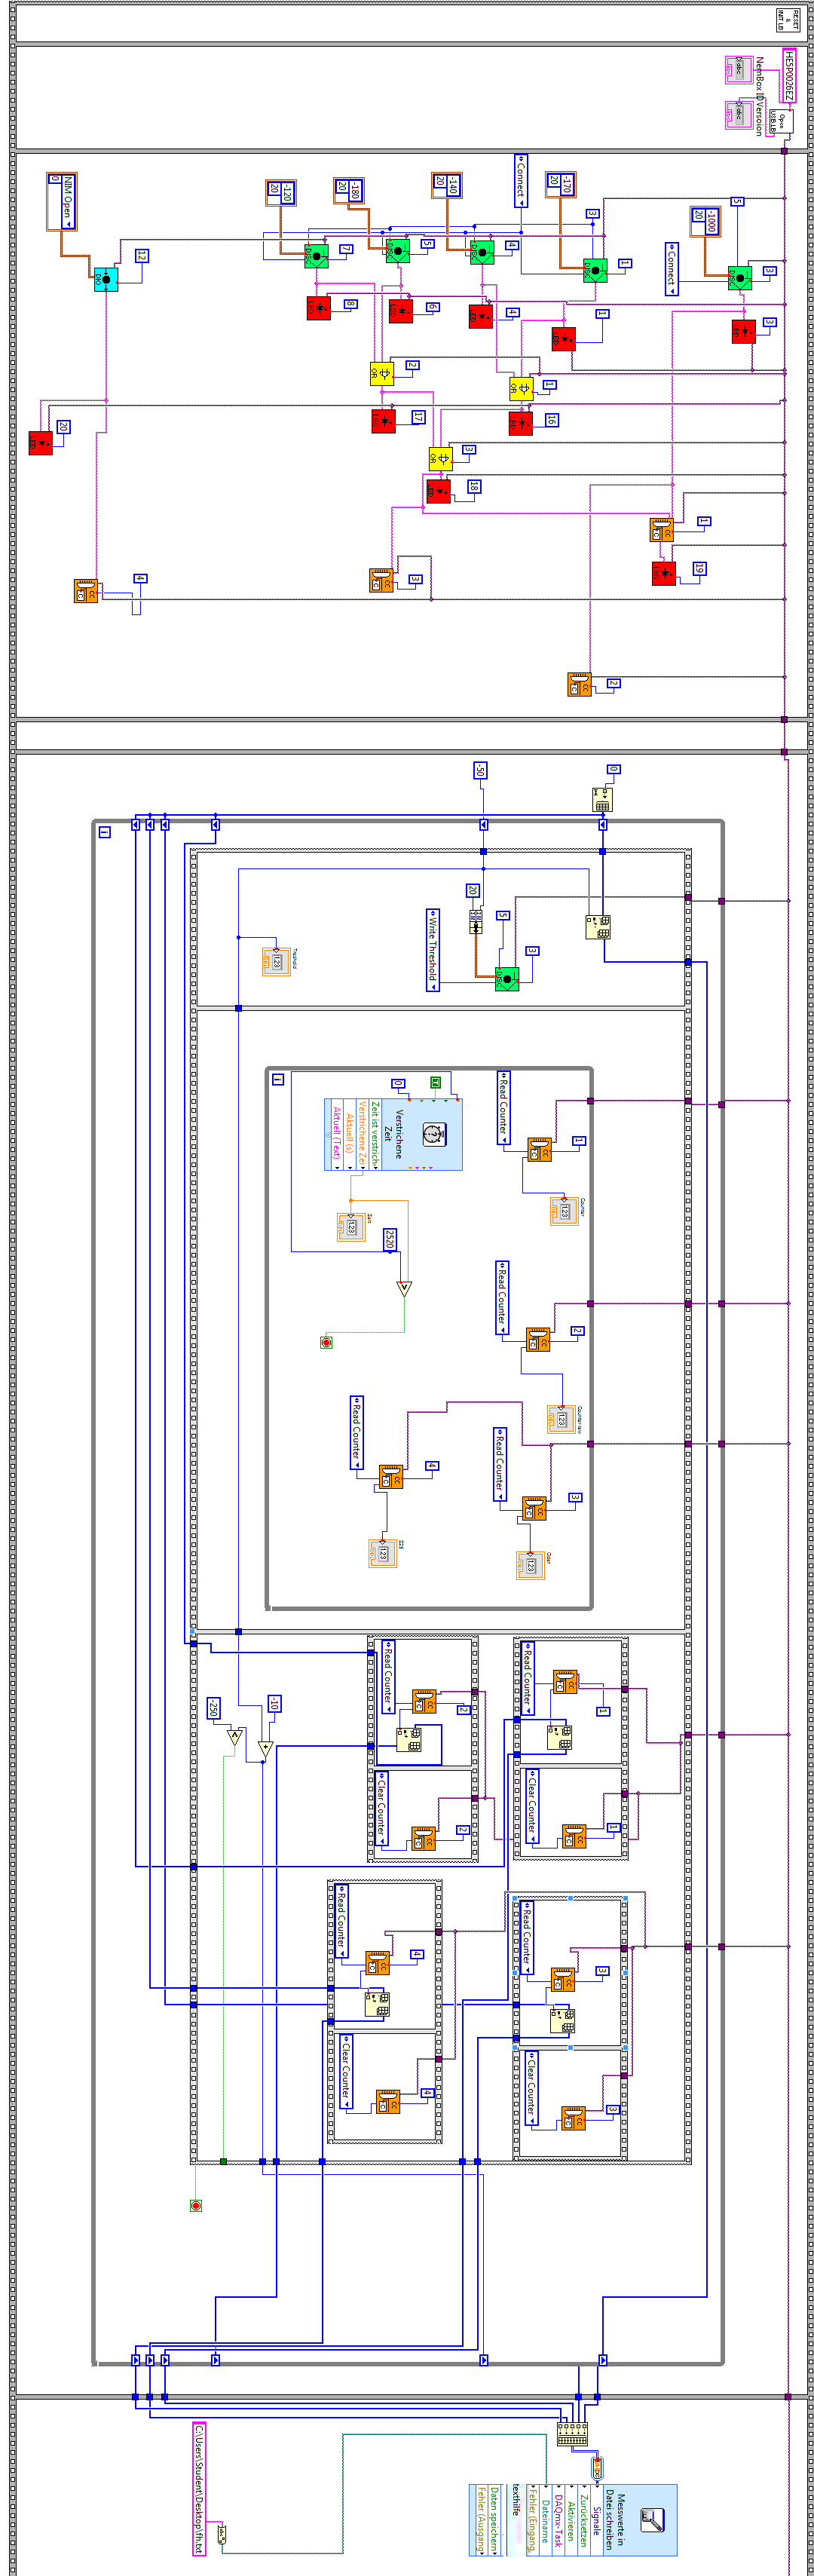
\includegraphics[height=20cm]{data/friedrich/prog_ges_rot.png}
\caption{Gesamtes Programm}
\label{fig:prog_all}
\end{figure}

\begin{figure}[h]
\centering
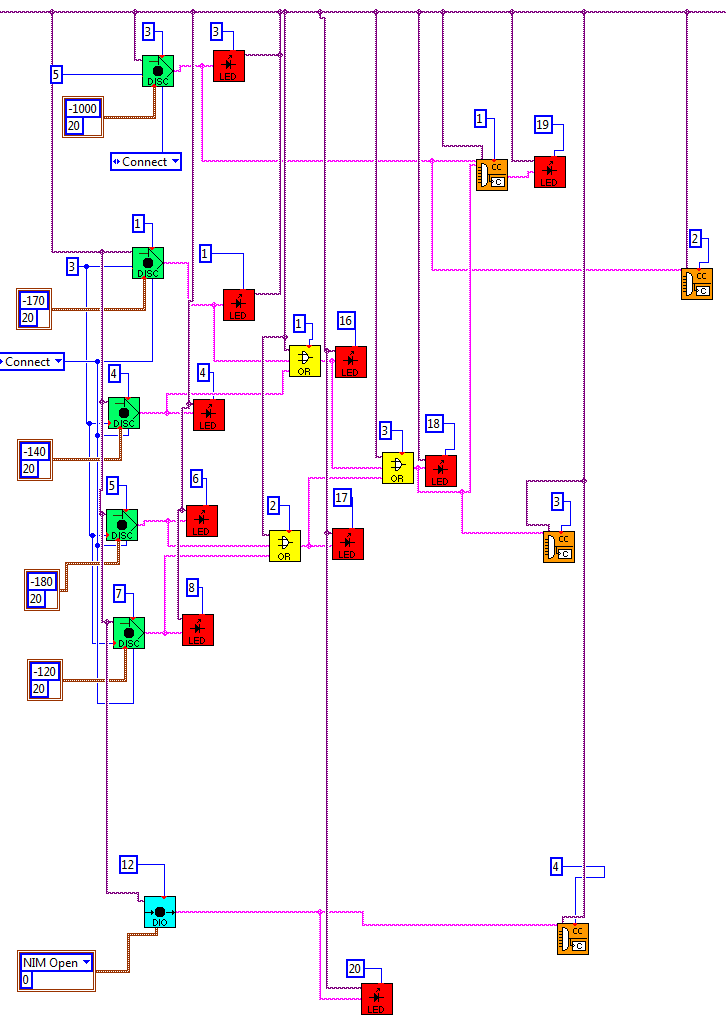
\includegraphics[height=20cm]{data/friedrich/prog_init.png}
\caption{Hardwareinitialisierung}
\label{fig:prog_init}
\end{figure}

\begin{figure}
\centering
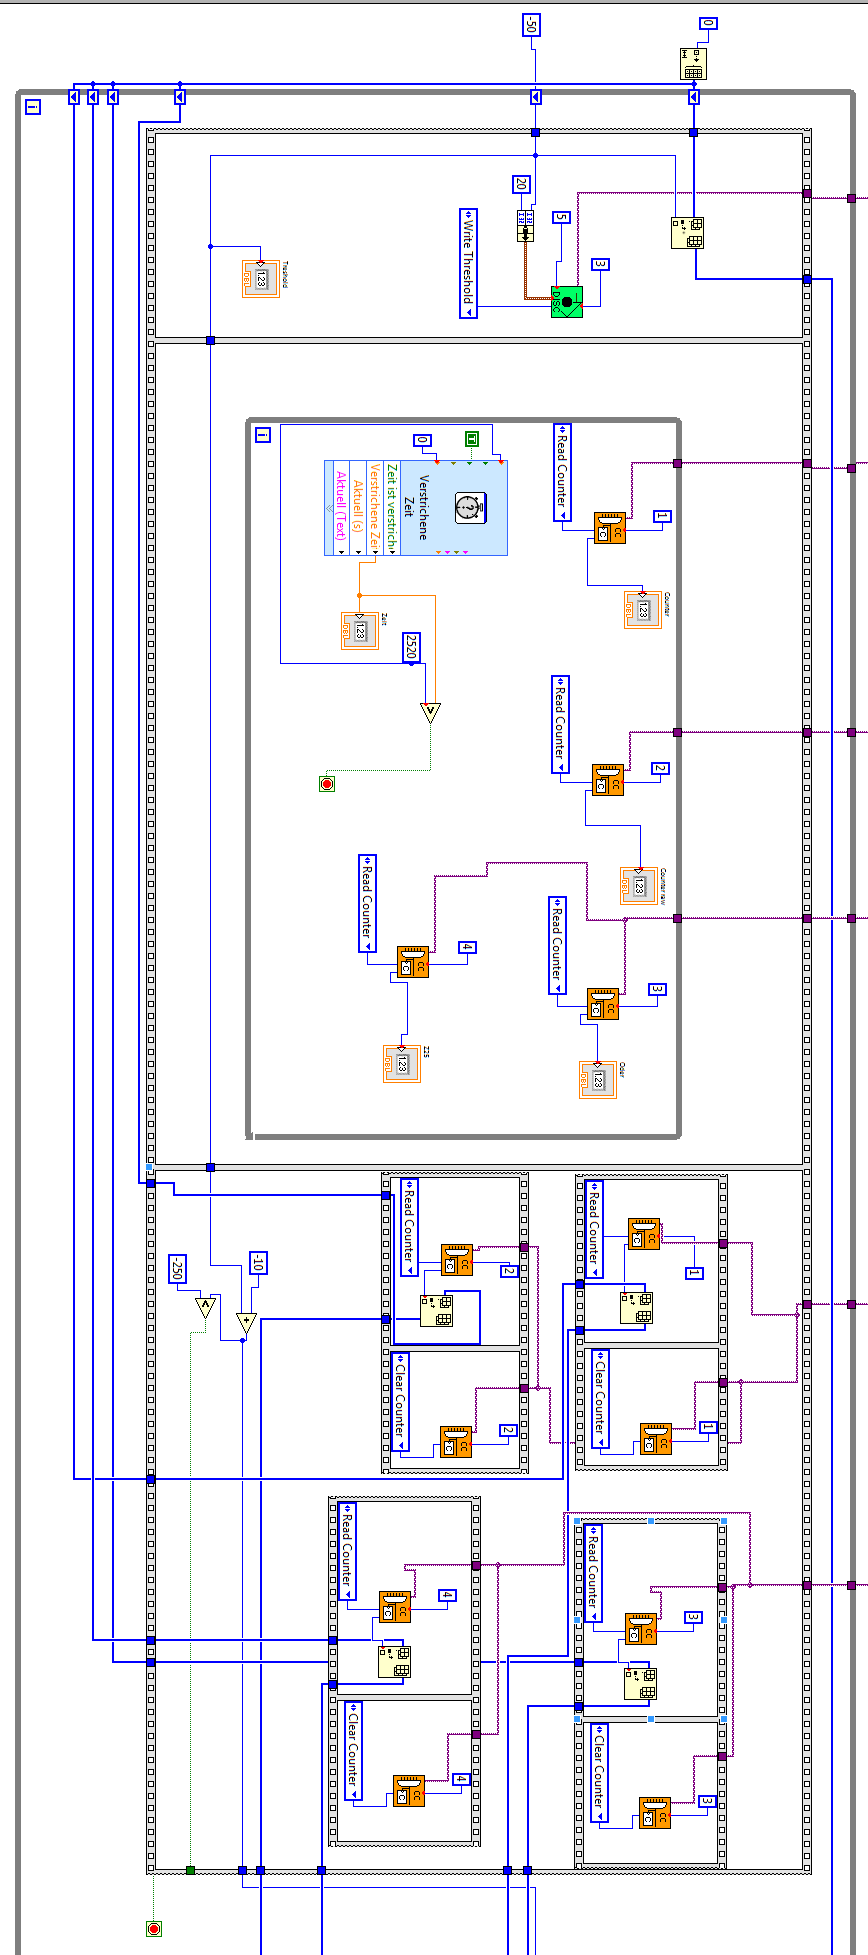
\includegraphics[height=20cm]{data/friedrich/prog_prog_rot.png}
\caption{Hauptprogramm}
\label{fig:prog_prog}
\end{figure}

\FloatBarrier

\subsubsection{Zufallskoinzidenzen}
Zusätzlich zur eigentlichen Messung wird versucht die Häufigkeit von Zufallskoinzidenzen zu messen. Dies geschieht auf 2 Arten.
\begin{itemize}
	\item Räumliche Zufallskoinzidenzen: Die Koinzidenzen von Detektor Z11, Z14 und Z25 werden gezählt. Solche Koinzidenzen werden z.B. verursacht von Teilchen, die nur in 2 Detektoren ein Signal auslösen, aber zufällig ein weiteres Signal in dem letzten Detektor erzeugt wird. Geht man von einem Teilchen aus, dass z.B. durch Z11 und Z25 geflogen ist, dann wird eine zufällige Koinzidenz erkannt, wenn 50ns davor oder danach ein Signal aus Z14 kommt. Die erwartete Rate beträgt also bei insgesamt N Ereignisse und einer Messdauer $t$ etwa: 
\begin{align}
N_{\text{raum}} = \frac{100\si{\nano\second}}{t} \cdot N
\label{equ:random_space}
\end{align}

	\item Zeitliche Zufallskoinzidenzen: Die Signale von Z2, Z14 und Z25 werden so verzögert, dass ein Teilchen keine Koinzidenz mehr erzeugen kann. Die Koinzidenzen, die dann gemessen werden, entsprechen 3 zufälligen Signalen in den Detektoren. Für eine Koinzidenz muss nun nicht nur ein Ereignis zufällig $50\si{\nano \second}$ vor oder $100 \si{\nano \second}$ nach dem Z25 Signal passiert sein, sondern auch noch ein weiteres Signal $30\si{\nano \second}$ vorher oder $50\si{\nano \second}$ danach. Die Rate beträgt also etwa:
	\begin{align}
N_{\text{zeit}} = \frac{150\si{\nano\second}}{t} \cdot N \cdot \frac{80\si{\nano\second}}{t} \cdot N = \frac{12000 \si{\nano\second}^2}{t^2}N^2
\label{equ:random_time}
\end{align}

\end{itemize}

\subsubsection{Pulshöhenspektrum}
Weiterhin wird auch noch die Energieverteilung der Teilchen in Z12 gemessen. Der Aufbau ist dabei so ähnlich wie bei der Messung der Schwellenkurve. Wieder zählen nur Ereignisse, die eine Koinzidenz aus D12 und D23, D24, D1 oder D2 darstellen. Kommt es zu einer solchen Koinzidenz wird das Signal in Z12 an einen MCA weitergeleitet, der die Ereignisse nach der Energie sortiert.

\section{Auswertung}
\subsection{Graphit}
\subsubsection{Grobe Struktur}
\begin{figure}
\centering
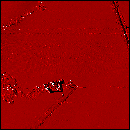
\includegraphics[scale=1]{data/graphit/raw_big.png}
\caption{Grobe Graphitstruktur (Seitenlänge 200nm)}
\label{fig:raw_big}
\end{figure}
In Abb. \ref{fig:raw_big} ist eine Aufnahme mit der Seitenlänge 200nm (CCM-Methode) dargestellt. Man kann eine grobe Struktur unten links, sowie mehrere Kanten erkennen.

\subsubsection{Atomare Auflösung}
Unsere Spitze war geeignet, um atomare Auflösung bei Graphit zu erreichen.
\begin{figure}
\centering
\includegraphics[scale=1]{data/graphit/raw.png}
\caption{Gemessene Graphitstruktur (Seitenlänge 4nm)}
\label{fig:raw}
\end{figure}
\begin{figure}
\centering
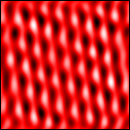
\includegraphics[scale=1]{data/graphit/2nm_edit2.png}
\caption{Graphitstruktur mit Fourierfilter}
\label{fig:edit}
\end{figure}
\begin{figure}
\centering
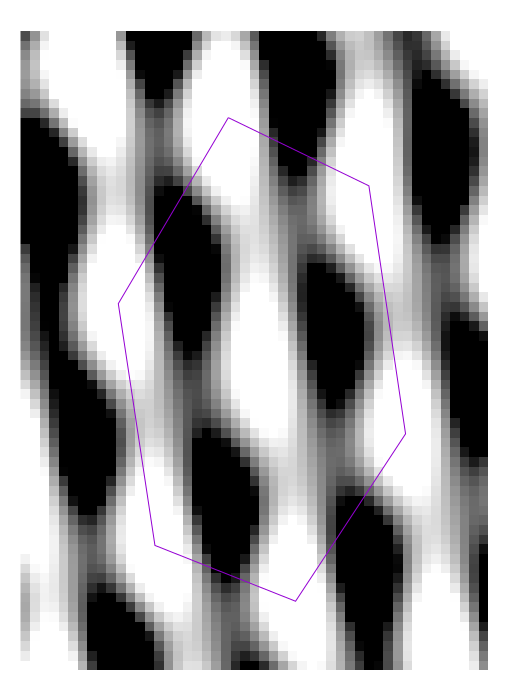
\includegraphics[scale=0.35]{data/graphit/graphit.png}
\caption{Ausschnitt mit ermittelten Mittelpunkten}
\label{fig:small}
\end{figure}
In Abb. \ref{fig:raw} ist das gemessene Bild (CHM-Methode) dargestellt. Da das Bild stark verrauscht ist, wurde ein Fourierfilter angewendet. Das Ergebnis ist in Abb. \ref{fig:edit} dargestellt. Man kann gut das sechseckige Gitter, dass die weißen Bereiche aufspannen, erkennen. Das sind die Punkte, in denen zwei Kohlenstoffatome übereinander liegen. Es handelt sich also nicht um die sechseckige Graphitstruktur, sondern nur um einen Teil davon. Für die Auswertung der Winkel können diese Punkte aber trotzdem verwendet werden, da die Winkel der Gitterstruktur gleich den Winkeln der Sechsecke sind.\\

In einem kleinem Ausschnitt (siehe Abb. \ref{fig:small}) wird nun ein solches Sechseck vermessen. Die Mittelpunkte der weißen Bereiche relativ zum weißem Bereich in der Mitte sind in Tab.\ref{tab:points} dargestellt (Fehler etwa $\Delta x,\Delta y=$ 0,01 nm).

\begin{table}
\centering
\caption{Bestimmte Mittelpunkte der weißen Bereiche}
\begin{tabular}{ccc}
\toprule
n & x/nm & y/nm\\
\midrule
1 & -0,05 &-0,41\\
2 & 0,18&	-0,3\\
3 & 0,24&	0,1\\
4 & 0,06&	0,37\\
5 & -0,17&	0,28\\
6 & -0,23&	-0,11\\
\bottomrule
\end{tabular}
\label{tab:points}
\end{table}
 
Die Punkte bilden offensichtlich kein regelmäßiges Sechseck. Das liegt daran, dass das Bild verzerrt wurde. Um es zu entzerren, drehen wir erst das Bild um den Winkel $\phi$, so dass die Verzerrungsachse in Richtung y-Achse zeigt. Dann verzerren wir das Bild in Richtung y-Achse um den Faktor $\alpha$. Die einzelnen Punkte sollten dann möglichst auf einem Kreis mit Radius $r$ liegen. Dazu sollte der Abstand aller der Punkte zum Ursprung etwa $r$ sein.\\

Um ein möglichst gutes Ergebnis zu erhalten, machen wir einen Fit über die freien Parameter $\phi, \alpha, r$, um die folgende Funktion zu minimieren:
\begin{align*}
f(\phi,\alpha,r) &= \sum\limits_{n = 1}^6 \left(\left|
\begin{pmatrix}
1 & 0\\
0 & \alpha
\end{pmatrix}
\begin{pmatrix}
\cos{\phi} & \sin{\phi}\\
-\sin{\phi} & \cos{\phi}
\end{pmatrix}
\begin{pmatrix}
x_n\\
y_n
\end{pmatrix}
  \right| - r\right)^2
\end{align*}.
Die rechte Matrix dreht das Polygon und die linke verzerrt die y-Achse. Danach wird von der Norm des Vektors $r$ abgezogen und das Quadrat dieser Abweichung aufsummiert. Somit soll sichergestellt werden, dass alle Punkte am Ende näherungsweise auf einem Kreis liegen. Dabei muss beachtet werden, dass das Original in einer Richtung gestaucht wurde. Somit muss $\alpha > 1$ (um die Stauchung rückgängig zu machen) gelten.\\
Der Fit (siehe Tab.\ref{tab:fit}, Abb. \ref{fig:fit1}, Abb. \ref{fig:fit2}) ergab: $\phi = 91,7^\circ \pm 0,9^\circ, \alpha = 1,6 \pm 0,2, r = 0,4\si{\nano\metre} \pm 0,02\si{\nano\metre}$.\\ 

\begin{table}
\centering
\caption{Punkte nach der Entzerrung}
\begin{tabular}{ccc}
\toprule
n & x/nm & y/nm\\
\midrule
1&	-0,40836&	0,101854\\
2&	-0,305142&	-0,281216\\
3& 0,0929292&	-0,399014\\
4&	0,368084&	-0,116354\\
5&	0,284858&	0,265753\\
6&	-0,103218&	0,38307\\
\bottomrule
\end{tabular}
\label{tab:fit}
\end{table}

\begin{figure}
\centering
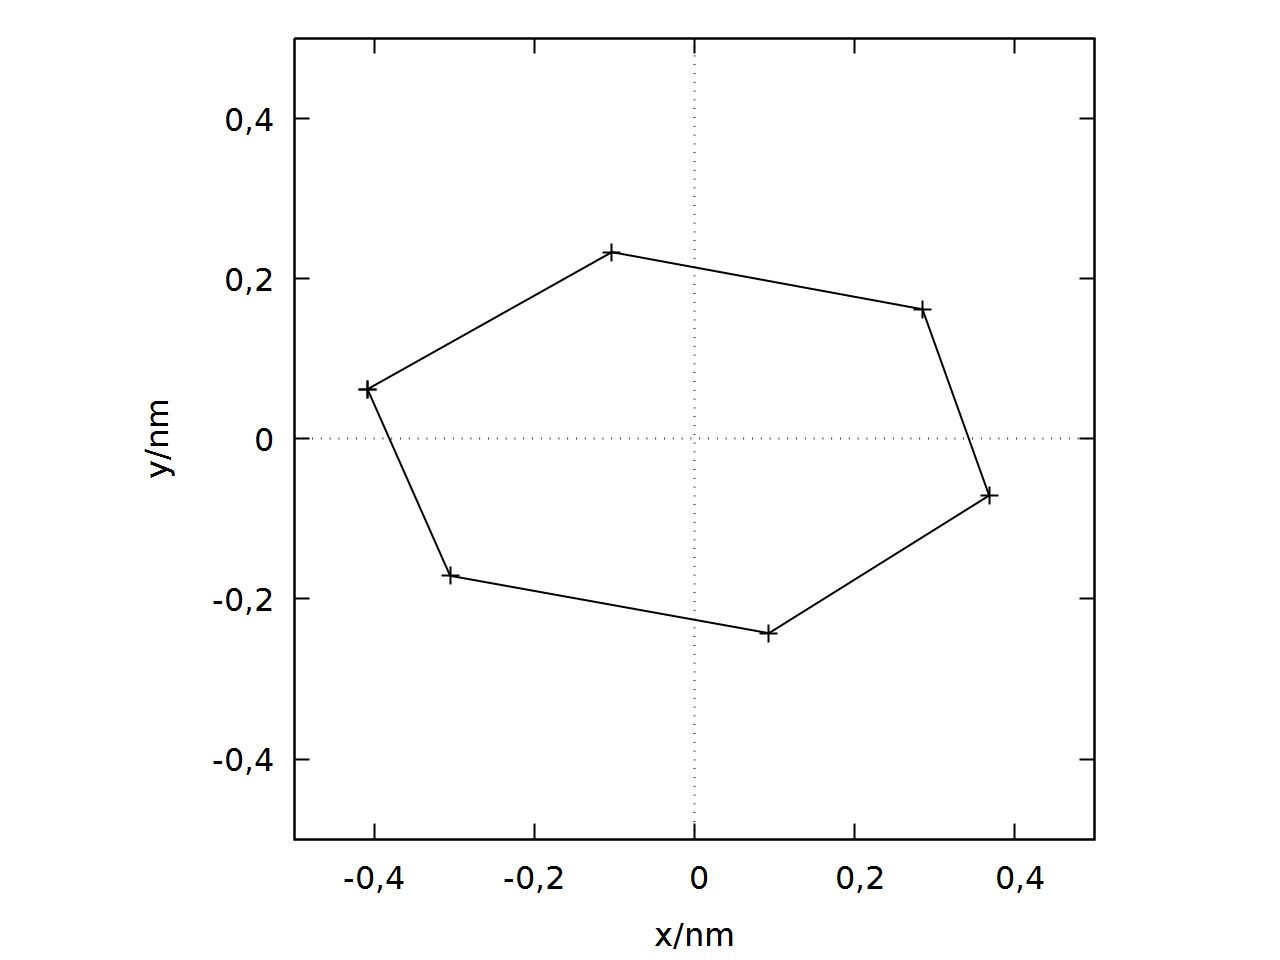
\includegraphics[scale=0.3]{data/graphit/out_rotate_old.png}
\caption{Nach Drehung um Winkel $\phi = 91,7^\circ$}
\label{fig:fit1}
\end{figure}

\begin{figure}
\centering
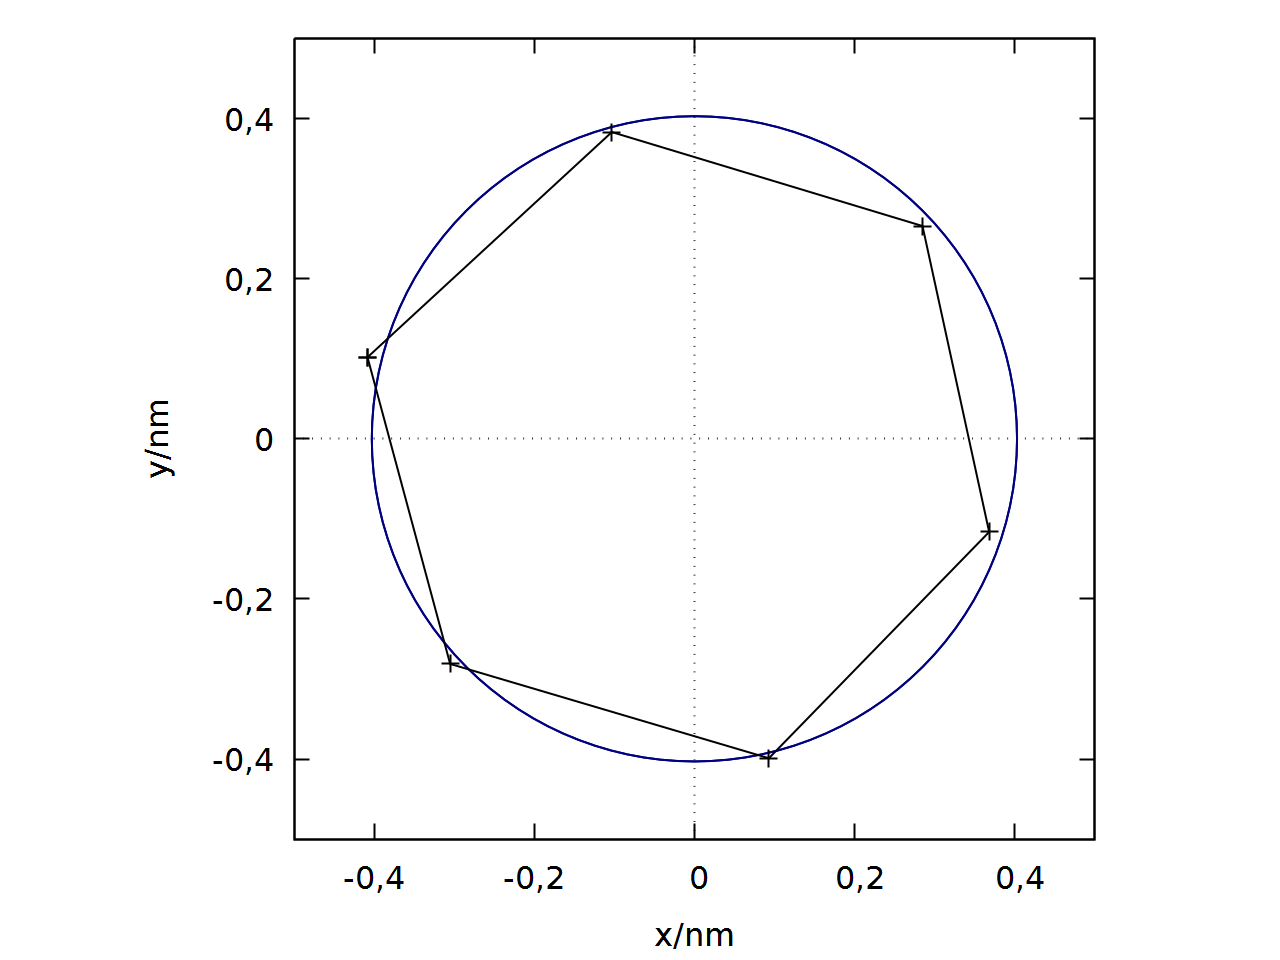
\includegraphics[scale=0.3]{data/graphit/out_rotate.png}
\caption{Nach Drehung und Entzerrung}
\label{fig:fit2}
\end{figure}

Wie man in Abb. \ref{fig:fit2} erkennt, liegen die Punkte jetzt fast auf einem Kreis, sie sind nur etwas verschoben. In Tab. \ref{tab:res} sind die gemessenen Kantenlängen und Innenwinkel aufgetragen. Durch Mittelung (Fehler über Standartabweichung) ergibt sich $l = 0,40 \pm 0,01$ und $\phi = 120^\circ \pm 2,3^\circ$. Dass der Wert für $\phi = 120^\circ$ beträgt, liegt nicht an einer genauen Messung, sondern daran, dass jedes Sechseck eine Innenwinkelsumme von $720^\circ$ hat. Demzufolge ist nur der Fehler ausschlaggebend. Bei $\Delta\phi=2,3^\circ$ kann man davon ausgehen, dass es sich um gleichseitige Sechsecke handelt und somit Graphit eine Gitterstruktur aus regelmäßigen Sechsecken hat.\\

\begin{table}
\centering
\caption{Punkte nach der Entzerrung}
\begin{tabular}{>{$}c<{$}cc}
\toprule
n & l/nm & $\phi/^\circ$\\
\midrule
1 \to 2 & 0,397 & 117,583\\
2 \to 3 & 0,415 & 121,565\\
3 \to 4 & 0,394 & 117,745\\
4 \to 5 & 0,391 & 123,483\\
5 \to 6 & 0,405 & 119,108\\
6 \to 1 & 0,415 & 120,516\\
\bottomrule
\end{tabular}
\label{tab:res}
\end{table}

Um die Atomabstände $a$ von Graphit zu bestimmen, muss beachtet werden, dass die weißen Punkte nur die Atome darstellen, die direkt über einem anderem sind. Drei benachbarte Atome in einem Sechseck bilden ein gleichschenkliges Dreieck mit der Basis $l$ und den Atomabständen $a$ als Schenkel (siehe Abb. \ref{fig:triangle}). Der Winkel an der Spitze beträgt $120^\circ$. Damit ergibt sich
\begin{align*}
a\cdot\sin{\frac{120^\circ}{2}} &= \frac{l}{2}\\
a &= \frac{l}{\sqrt{3}}\\
  &= 0,231 \pm 0,006
\end{align*}. Der Abstand der Atome beträgt also $a = 0,231\si{\nano\metre} \pm 0,006\si{\nano\metre}$.

\begin{figure}
\centering
\definecolor{qqwuqq}{rgb}{0.,0.39215686274509803,0.}
\definecolor{ffffff}{rgb}{1.,1.,1.}
\begin{tikzpicture}[line cap=round,line join=round,>=triangle 45,x=3.0cm,y=3.0cm]
\clip(-1.798235627638573,-1.1694768704984821) rectangle (2.968878775383718,1.243097549118033);
\draw [shift={(0.,0.)},color=qqwuqq,fill=qqwuqq,fill opacity=0.10000000149011612] (0,0) -- (-60.:0.12435950616579888) arc (-60.:0.:0.12435950616579888) -- cycle;
\draw (-0.5,0.8660254037844388)-- (0.5,0.8660254037844386);
\draw (0.5,0.8660254037844386)-- (1.,0.);
\draw (1.,0.)-- (0.5,-0.866025403784439);
\draw (0.5,-0.866025403784439)-- (-0.5,-0.8660254037844384);
\draw (-0.5,-0.8660254037844384)-- (-1.,0.);
\draw (-1.,0.)-- (-0.5,0.8660254037844388);
\draw [dash pattern=on 1pt off 1pt] (0.5,0.8660254037844386)-- (1.5,0.866025403784439);
\draw [dash pattern=on 1pt off 1pt] (0.5,0.8660254037844386)-- (0.,0.);
\draw [dash pattern=on 1pt off 1pt] (0.,0.)-- (0.5,-0.866025403784439);
\draw [dash pattern=on 1pt off 1pt] (0.5,-0.866025403784439)-- (1.5,-0.8660254037844395);
\draw [dash pattern=on 1pt off 1pt] (1.5,-0.8660254037844395)-- (2.,0.);
\draw [dash pattern=on 1pt off 1pt] (1.5,0.866025403784439)-- (2.,0.);
\draw [dotted] (0.5,0.8660254037844385)-- (0.5,-0.8660254037844392);
\draw [dotted] (0.,0.)-- (0.5,0.);
\begin{scriptsize}
\draw [fill=ffffff] (0.,0.) circle (2.5pt);
\draw[color=black] (0.2039524216307892,0.5031584874315245) node {a};
\draw[color=black] (0.2039524216307892,-0.4295378088119736) node {a};
\draw [fill=ffffff] (0.5,0.8660254037844385) circle (2.5pt);
\draw[color=ffffff] (0.5272871376618663,0.9425620758840169) node {$E$};
\draw [fill=ffffff] (0.5,-0.8660254037844392) circle (2.5pt);
\draw[color=ffffff] (0.5272871376618663,-0.790180376692793) node {$F$};
\draw [fill=ffffff] (-1.,0.) circle (2.5pt);
\draw[color=ffffff] (-0.9691722531999137,0.07619084959561201) node {$G$};
\draw [fill=ffffff] (2.,0.) circle (2.5pt);
\draw[color=ffffff] (2.02789184539584,0.07619084959561201) node {$H$};
\draw[color=black] (0.5314324545340595,-0.031587389081414445) node {l};
\draw [fill=ffffff] (1.,0.) circle (2.5pt);
\draw[color=ffffff] (1.041306429813835,0.07619084959561201) node {$F'$};
\draw[color=qqwuqq] (0.08788354920937688,-0.019151438464834462) node {60\textrm{\degre}};
\end{scriptsize}
\end{tikzpicture}
\caption{Zwei Sechsecke in unterschiedlichen Ebenen}
\label{fig:triangle}
\end{figure}


\subsection{Gold}
\begin{figure}
\centering
\includegraphics[scale=1]{data/gold/raw.png}
\caption{Grobe Goldstruktur (Seitenlänge 100nm)}
\label{fig:gold}
\end{figure}
In Abb. \ref{fig:gold} ist eine Aufnahme mit der Seitenlänge 100nm (CCM-Methode) dargestellt.  Da der linke Teil deutlich heller ist, ist er höher als der rechte. Wir denken also, dass die Aufnahme an einer Kante entstanden ist. Im Vergleich zu Graphit wirkt die Aufnahme verschwommen und es bilden sich wolkenartige Strukturen. Dies liegt daran, dass die Ladungsdichte in Gold deutlich homogener verteilt ist als in Graphit. Demzufolge war es uns auch nicht möglich eine Aufnahme mit atomarer Auflösung herzustellen. Um die atomare Oberfläche von Gold zu betrachten, bräuchte man eine andere Methode, wie z.B. ein Rasterkraftmikroskop.

\subsection{TaS$_2$}
\begin{figure}
\centering
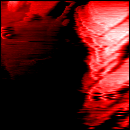
\includegraphics[scale=1]{data/tas2/tas2.png}
\caption{Grobe TaS$_2$-Struktur (Seitenlänge 84,7nm)}
\label{fig:tas2}
\end{figure}
In Abb. \ref{fig:tas2} ist eine Aufnahme mit der Seitenlänge 84,7nm (CCM-Methode) dargestellt. Auch hier kann man grobe Strukturen erkennen, die höher liegen als andere. Eine Abbildung mit atomarer Auflösung aufzunehmen war leider nicht möglich. Demzufolge konnten wir auch keine Ladungsdichtewellen erkennen. 

\section{Frank-Hertz-Versuch}
\subsection{Theoretische Vorbetrachtungen}
Beim Photoeffekt treffen Photonen auf eine Photozelle. In der Photozelle befinden sich (getrennt voneinander) eine Anode und eine Kathode. Diese sind an eine äußere Spannung $U_\mathrm{G}>0$ angeschlossen. Betrachtet man die Elektronen im Bändermodell, so führt die Verbindung mit der Spannungsquelle dazu, dass die Fermie-Niveaus von Anode ($E_\mathrm{FA}$) und Kathode ($E_\mathrm{FK}$) nun eine Potentialdifferenz von $e U_\mathrm{G}$ haben, wobei $e$ die Elementarladung ist. Bei unterschiedlichen Austrittsarbeiten $W_\mathrm{A}$ und $W_\mathrm{K}$ von Anode und Kathode entsteht eine Potentialdifferenz von $eU_\mathrm{AK}=W_\mathrm{A}-W_\mathrm{K}$, das so genannte Kontaktpotential (siehe Abbildung \ref{Photozelle}). 

\begin{figure}[h]
  \centering
  \begin{tikzpicture}
    \draw (0,0)--(2,0);
    \draw (-0.4,0) node {$E_\mathrm{FK}$};
    \draw (2,1)--(4,1);
    \draw (4.4,1) node {$E_\mathrm{FA}$};
    \draw [<->] (2,0.1)--(2,0.9);
    \draw (2.5,0.5) node {$eU_\mathrm{G}$};
    \draw [<->] (0.3,0.1)--(0.3,1.9);
    \draw (-0.1,1) node {$W_\mathrm{K}$};
    \draw [<->] (3.7,1.1)--(3.7,3.9);
    \draw (4,2.5) node {$W_\mathrm{A}$};
    \draw [thick, dash dot] (0,2)--(2,2);
    \draw [thick, dash dot] (2,4)--(4,4);
    \draw [<->] (2,2.1) --(2,3.9);
    \draw (1.4,3) node {$eU_\mathrm{KA}$};
    \draw (-0.5,-0.3)--(-0.5,-1);
    \draw (-0.5,-1)--(1.5,-1);
    \draw (4.3,0.7)--(4.3,-1);
    \draw (4.3,-1)--(2.5,-1);
    \draw (1.55,-1) circle (0.05cm);
    \draw (1.55,-1.3) node {$+$};
    \draw (2.45,-1) circle (0.05cm);
    \draw (2.45,-1.3) node {$-$};
    \draw (2,-1) node {$U_\mathrm{G}$};
  \end{tikzpicture}
  \caption{Energieniveaus in Photozelle}
  \label{Photozelle}
\end{figure}

Damit nun ein gebundenes Elektron der Kathode zu der Anode gelangen kann muss es die Potentialdifferenz $W_\mathrm{A}+eU_\mathrm{G}$ überwinden. Ein einzelnes Photon hat eine von der Frequenz $\nu$ abhängige Energie von $E=h\nu$, wobei $h$ das Plancksche Wirkungsquantum ist. Reicht diese Energie aus, um die Potentialdifferenz zwischen Kathode und Anode zu überwinden, so kann ein Strom zwischen den Elektroden fließen. Bei der Grenzspannung $U_0$ ist die Energie der Photonen gerade so groß, dass ein kleiner Strom fließen kann. Dann folgt die Energiebilanz
\begin{align}
  h\nu=eU_0+W_\mathrm{A}.
  \label{eqn:grenzspannung}	
\end{align}
Hierbei wird angenommen, dass $W_\mathrm{A}+eU_\mathrm{G} \geq W_\mathrm{K}$ gilt. Ist dies nicht der Fall, müsste lediglich die Potentialdifferenz $W_\mathrm{K}$ überwunden werden und $W_\mathrm{K}$ könnte bestimmt werden. \\ \\
Aus \cite{kennlinie} folgt (mit $h\nu>eU_\mathrm{G}+w_\mathrm{A}$), dass bei kleinen Temperaturen für die Zahl der herausgelösten Elektronen $N$ und den Photostrom $I$
\begin{align}
  I \propto N \propto \left(  h\nu-W_\mathrm{A}-eU_\mathrm{G}\right)^2
\end{align} 
gilt. 

\section{Durchführung}

\\ \\
\subsection{Bestimmung der Lebensdauer}
Für die Bestimmung der Lebensdauer sind zwei Fehler relevant. Zum einen der statistische Fehler durch die Poissonverteilung der Zählwerte und zum anderen die Zahl der Zufallsereignisse. Die Zahl der Zufallsereignisse trägt für jedes der zehn Zählintervalle gleich bei, da keine zeitliche Korrelation besteht. Somit wird bei der Auftragung der Zählereignisse gegen die Zeit die Form

\begin{align}
  N(t)=A e^{-t/\tau}+B
  \label{eq:fit_lebensdauer}
\end{align}
 erwartet. $B$ entsteht dabei durch die Zahl der Zufallsereignisse pro Sichtzähler.
Insgesamt wurden $N_s=2054703$ Startsignale ausgelöst. Da der Teil der Startsignale, der auch zu einer Zählung eines Myonenzerfalls geführt hat, verschwindend gering ist, folgt, dass das Gate für die Messung ungefähr $N_s \cdot \SI{10}{\micro\second}\approx\SI{20.5}{\second}$ geöffnet war. Die Zahl der Zufallsereignisse lässt sich nun durch Multiplikation mit der Rate an Stopsignalen berechnen. Es wurden in der gesamten Zeit von 13 Tagen und 2 Stunden 4314850 Stopsignale ausgelöst. Somit folgt für die Zahl der Zufallsereignisse 
\begin{align*}
  N_z\approx 78.
\end{align*}
Diese Abschätzung kann durch Anpassung der Funktion (\ref{eq:fit_lebensdauer}) mit dem erhaltenen $B$ verglichen werden. Aus der Anpassung folgt
\begin{align*}
  A&=1621 \pm 80\\
  \tau&=\SI[separate-uncertainty = true]{2.2(1)}{\micro\second}\\
  B&=9 \pm 7.
\end{align*}
Da es zehn Sichtzähler gibt gilt im Idealfall $N_z=10B$. Dies stimmt auch grob, allerdings ist der Fehler von $B$ aufgrund der geringen Zählraten fast so groß wie $B$ selbst. Die Lebensdauer von Myonen wurde zu $\tau = \SI[separate-uncertainty = true]{2.2(1)}{\micro\second}$ bestimmt. Die Auftragung der Daten sowie die Anpassungskurve sind in Abbildung \ref{fig:lebensdauer} zu sehen. Die Daten befinden sich in Tabelle \ref{tab:sichtzaehler}.

\begin{figure}[h]
  \centering
  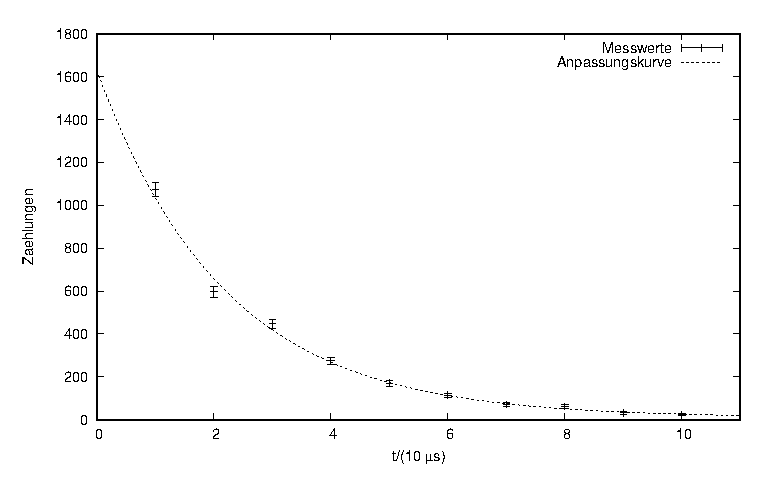
\includegraphics[width=0.8\textwidth]{./data/lebensdauer.eps}
  \caption{Kurve zur Messung der Lebensdauer von Myonen}
  \label{fig:lebensdauer}
\end{figure}


\begin{table}[h]
    \centering
    \caption{abgelesene Zählereignisse von Sichtzählern zur Lebensdauerbestimmung}
    \label{tab:sichtzaehler}
    \begin{tabular}{c | c c c c c c c c c c}
      Sichtzähler &1&2&3&4&5&6&7&8&9&10\\ \hline
      Zählungen &1072&596&447&274&170&114&71&61&32&25\\
    \end{tabular}
  \end{table}



\section{Fazit}
Wir haben Bilder von der Oberfläche von Graphit, Gold und TaS$_2$ in der Größenordung von 100nm aufgenommen. Zusätzlich war es möglich ein Bild der Graphitoberfläche mit atomarer Auflösung zu erstellen. Mithilfe dieses Aufnahme konnten wir (nach Entzerrung des Bildes) bestätigen, dass die Bindungswinkel der Graphitstruktur $120^\circ \pm 2,3^\circ$ beträgt, es sich also um eine Struktur aus regelmäßigen Sechsecken handelt. Der Atomabstand wurde zu $a = 0,231\si{\nano\metre} \pm 0,006\si{\nano\metre}$ bestimmt.    

\newpage
\section{Anhang}
\begin{table}
\centering
\caption{Fitparameter und berechnete Gangunterschiede}
\ref{tab:werte}
\begin{tabular}{S[round-mode=places,round-precision=1]S[round-mode=places,round-precision=0]S[round-mode=places,round-precision=2]S[round-mode=places,round-precision=2]S[round-mode=places,round-precision=2]S[round-mode=places,round-precision=2]S[round-mode=places,round-precision=2]S[round-mode=places,round-precision=2]S[round-mode=places,round-precision=9]S[round-mode=places,round-precision=2]}
{$I/\si{\ampere}$}	&	{n}	&	{$a/\%$}	&	{$\Delta a/\%$}	&	{$b$}	&	{$\Delta b$}	&	{$s$}	&	{$\Delta s$}	&	{$g/\si{\si{m}}$}	&	{$\Delta g/\si{\meter}$}\\
\toprule
6	&	1	&	28,5016	&	0,849783	&	829,358	&	0,492301	&	12,95453556	&	0,704329829	&	0,011655094	&	4,58358E-09\\
6	&	2	&	21,1055	&	1,16465	&	849,878	&	0,187483	&	4,834382153	&	0,247274946	&	0,011655275	&	1,56152E-09\\
6	&	3	&	38,5883	&	0,293881	&	871,119	&	0,534864	&	19,33226282	&	0,704277171	&	0,011655441	&	3,91131E-09\\
6	&	4	&	21,6083	&	0,782926	&	921,91	&	0,35641	&	13,000314	&	0,459584163	&	0,011655751	&	1,74039E-09\\
6	&	5	&	51,5363	&	0,462747	&	979,654	&	0,684621	&	32,27108592	&	0,92221909	&	0,011655953	&	1,45215E-09\\
6	&	6	&	51,7062	&	0,356072	&	1065,99	&	0,729291	&	34,32797346	&	0,989290033	&	0,011655958	&	1,46471E-09\\
6	&	7	&	20,074	&	0,738264	&	1125,08	&	0,323965	&	12,08075329	&	0,429837517	&	0,011655756	&	1,56631E-09\\
6	&	8	&	34,5089	&	0,302	&	1174,27	&	0,616481	&	18,09819824	&	0,699844561	&	0,01165546	&	4,43115E-09\\
6	&	9	&	27,9089	&	1,64872	&	1195,93	&	0,22516	&	6,153073153	&	0,272019088	&	0,011655293	&	1,85171E-09\\
6	&	10	&	28,7849	&	0,674773	&	1216,72	&	0,378693	&	11,12059499	&	0,480340739	&	0,011655112	&	3,49101E-09\\
\midrule
6,3	&	1	&	31,387	&	0,903664	&	829,069	&	0,574861	&	14,16337527	&	0,755105684	&	0,011655091	&	5,36021E-09\\
6,3	&	2	&	21,2711	&	1,1059	&	850,298	&	0,178191	&	4,835910933	&	0,238872606	&	0,011655278	&	1,48054E-09\\
6,3	&	3	&	41,3403	&	0,327233	&	871,999	&	0,567802	&	19,46178439	&	0,77409482	&	0,011655447	&	4,12827E-09\\
6,3	&	4	&	24,7343	&	0,851412	&	921,952	&	0,358973	&	13,3563497	&	0,448894599	&	0,011655751	&	1,75218E-09\\
6,3	&	5	&	54,4236	&	0,611898	&	979,675	&	0,729286	&	31,71724317	&	0,915764245	&	0,011655953	&	1,54615E-09\\
6,3	&	6	&	55,7872	&	0,389607	&	1064,36	&	0,779025	&	34,96972101	&	1,041599763	&	0,011655961	&	1,50386E-09\\
6,3	&	7	&	22,6951	&	0,813742	&	1125,32	&	0,340425	&	12,76683544	&	0,45117248	&	0,011655754	&	1,64979E-09\\
6,3	&	8	&	37,0904	&	0,308758	&	1172,36	&	0,518518	&	17,17846766	&	0,687165036	&	0,011655474	&	3,67963E-09\\
6,3	&	9	&	32,5284	&	1,88681	&	1195,29	&	0,219756	&	6,567635617	&	0,265695037	&	0,011655298	&	1,80054E-09\\
6,3	&	10	&	32,4417	&	0,500637	&	1216,77	&	0,373865	&	11,63001821	&	0,50501014	&	0,011655111	&	3,4474E-09\\
\midrule
6,6	&	1	&	32,9667	&	0,837135	&	828,568	&	0,523639	&	14,07784857	&	0,754080552	&	0,011655087	&	4,89515E-09\\
6,6	&	2	&	22,9343	&	1,25389	&	850,404	&	0,187006	&	5,14689011	&	0,251028949	&	0,011655279	&	1,55284E-09\\
6,6	&	3	&	41,9592	&	0,314762	&	872,619	&	0,520596	&	19,21310297	&	0,800620839	&	0,011655452	&	3,76961E-09\\
6,6	&	4	&	25,9236	&	0,8841	&	921,446	&	0,377889	&	13,44586822	&	0,459544245	&	0,011655748	&	1,85366E-09\\
6,6	&	5	&	55,8408	&	0,583553	&	980,444	&	0,747632	&	32,03174704	&	0,933795347	&	0,011655955	&	1,55755E-09\\
6,6	&	6	&	56,2759	&	0,439048	&	1064,42	&	0,787264	&	34,0842181	&	1,018642594	&	0,011655961	&	1,52203E-09\\
6,6	&	7	&	24,7069	&	0,822702	&	1125,89	&	0,36283	&	13,15947691	&	0,46998241	&	0,011655752	&	1,76827E-09\\
6,6	&	8	&	37,4038	&	0,308416	&	1171,1	&	0,456895	&	16,40779306	&	0,702014578	&	0,011655483	&	3,21479E-09\\
6,6	&	9	&	36,0039	&	1,99397	&	1195,1	&	0,222528	&	6,849007436	&	0,265326432	&	0,0116553	&	1,82123E-09\\
6,6	&	10	&	33,6566	&	0,401879	&	1217,24	&	0,362931	&	11,62730038	&	0,525996881	&	0,011655107	&	3,35474E-09\\
\midrule
6,9	&	1	&	34,9489	&	0,790265	&	828,234	&	0,483548	&	14,035977	&	0,747562007	&	0,011655083	&	4,52809E-09\\
6,9	&	2	&	24,699	&	1,40797	&	850,528	&	0,193453	&	5,405551064	&	0,259990143	&	0,01165528	&	1,60522E-09\\
6,9	&	3	&	43,2783	&	0,312716	&	873,167	&	0,47974	&	18,9233993	&	0,820184117	&	0,011655456	&	3,4612E-09\\
6,9	&	4	&	27,6339	&	0,926272	&	921,057	&	0,394872	&	13,61607231	&	0,46921802	&	0,011655747	&	1,94431E-09\\
6,9	&	5	&	57,3809	&	0,640938	&	980,383	&	0,759464	&	31,74586532	&	0,928036945	&	0,011655955	&	1,58441E-09\\
6,9	&	6	&	58,0811	&	0,452129	&	1063,81	&	0,803813	&	34,23327408	&	1,036121637	&	0,011655962	&	1,53057E-09\\
6,9	&	7	&	26,2347	&	0,853151	&	1126,35	&	0,382387	&	13,43644074	&	0,491045591	&	0,011655749	&	1,87199E-09\\
6,9	&	8	&	38,5257	&	0,315227	&	1170,26	&	0,415746	&	15,8111445	&	0,698357398	&	0,011655488	&	2,90855E-09\\
6,9	&	9	&	38,9209	&	2,09986	&	1194,88	&	0,225543	&	7,062110769	&	0,267110008	&	0,011655302	&	1,84353E-09\\
6,9	&	10	&	35,0754	&	0,366594	&	1217,52	&	0,36928	&	11,77126042	&	0,556452712	&	0,011655104	&	3,41837E-09\\
\midrule
7,2	&	1	&	38,302	&	0,708121	&	828,184	&	0,56175	&	15,21712883	&	0,8582142	&	0,011655083	&	5,26174E-09\\
7,2	&	2	&	26,0178	&	1,5707	&	850,905	&	0,200594	&	5,652007264	&	0,275845282	&	0,011655283	&	1,66086E-09\\
7,2	&	3	&	45,8882	&	0,375954	&	874,16	&	0,486584	&	18,29218334	&	0,854689514	&	0,011655463	&	3,48746E-09\\
7,2	&	4	&	30,1839	&	1,03816	&	920,77	&	0,427836	&	13,93286934	&	0,499785961	&	0,011655745	&	2,1125E-09\\
7,2	&	5	&	61,1654	&	0,712664	&	981,081	&	0,817231	&	32,09145436	&	0,987837693	&	0,011655956	&	1,67764E-09\\
7,2	&	6	&	61,7975	&	0,55241	&	1063,86	&	0,849066	&	33,86432869	&	1,072183841	&	0,011655962	&	1,61877E-09\\
7,2	&	7	&	29,2271	&	0,917013	&	1127,07	&	0,396656	&	14,04514968	&	0,527519715	&	0,011655746	&	1,95551E-09\\
7,2	&	8	&	41,2495	&	0,32468	&	1169,45	&	0,356187	&	14,78983503	&	0,648990569	&	0,011655494	&	2,47808E-09\\
7,2	&	9	&	44	&	2,23267	&	1194,55	&	0,22516	&	7,294510694	&	0,264115299	&	0,011655304	&	1,83685E-09\\
7,2	&	10	&	37,9037	&	0,358754	&	1217,76	&	0,387836	&	12,05111196	&	0,600131633	&	0,011655102	&	3,59459E-09\\
\bottomrule
\end{tabular}
\end{table}

\begin{table}\ContinuedFloat
\centering
\begin{tabular}{S[round-mode=places,round-precision=1]S[round-mode=places,round-precision=0]S[round-mode=places,round-precision=2]S[round-mode=places,round-precision=2]S[round-mode=places,round-precision=2]S[round-mode=places,round-precision=2]S[round-mode=places,round-precision=2]S[round-mode=places,round-precision=2]S[round-mode=places,round-precision=9]S[round-mode=places,round-precision=2]}
{$I/\si{\ampere}$}	&	{n}	&	{$a/\%$}	&	{$\Delta a/\%$}	&	{$b$}	&	{$\Delta b$}	&	{$s$}	&	{$\Delta s$}	&	{$g/\si{\si{m}}$}	&	{$\Delta g/\si{\meter}$}\\
\toprule
7,5	&	1	&	41,2826	&	0,680767	&	828,008	&	0,545552	&	15,36465603	&	0,896501626	&	0,011655081	&	5,11461E-09\\
7,5	&	2	&	28,3209	&	1,87001	&	851,149	&	0,214097	&	5,950348533	&	0,296231553	&	0,011655285	&	1,77016E-09\\
7,5	&	3	&	48,3495	&	0,395294	&	874,763	&	0,462635	&	17,95763548	&	0,892773104	&	0,011655467	&	3,30247E-09\\
7,5	&	4	&	32,5046	&	1,17099	&	920,533	&	0,467175	&	14,18902479	&	0,536565842	&	0,011655744	&	2,31204E-09\\
7,5	&	5	&	64,4808	&	0,808608	&	981,499	&	0,884953	&	32,25817623	&	1,056649745	&	0,011655957	&	1,79897E-09\\
7,5	&	6	&	65,0908	&	0,661405	&	1063,61	&	0,908542	&	33,63229397	&	1,130311425	&	0,011655962	&	1,72129E-09\\
7,5	&	7	&	31,8436	&	0,997837	&	1127,42	&	0,416964	&	14,53962483	&	0,568136832	&	0,011655744	&	2,06261E-09\\
7,5	&	8	&	43,5807	&	0,342122	&	1168,81	&	0,324144	&	14,21195648	&	0,623659546	&	0,011655498	&	2,24522E-09\\
7,5	&	9	&	46,1835	&	2,43014	&	1194,05	&	0,220252	&	7,360375599	&	0,266090821	&	0,011655308	&	1,79154E-09\\
7,5	&	10	&	40,1569	&	0,368355	&	1217,84	&	0,438522	&	13,16780026	&	0,679554263	&	0,011655101	&	4,06605E-09\\
\midrule
7,8	&	1	&	44,3432	&	0,594238	&	827,832	&	0,504399	&	15,39828917	&	0,923178824	&	0,01165508	&	4,73305E-09\\
7,8	&	2	&	31,74	&	2,31542	&	851,42	&	0,229708	&	6,366235939	&	0,318516059	&	0,011655288	&	1,89626E-09\\
7,8	&	3	&	50,5466	&	0,400049	&	875,54	&	0,417655	&	17,35699511	&	0,897130124	&	0,011655473	&	2,96586E-09\\
7,8	&	4	&	35,0287	&	1,26995	&	920,192	&	0,501846	&	14,45511731	&	0,570512385	&	0,011655742	&	2,49181E-09\\
7,8	&	5	&	67,6685	&	0,890704	&	981,874	&	0,929589	&	32,3045492	&	1,100313379	&	0,011655958	&	1,87304E-09\\
7,8	&	6	&	67,8515	&	0,754651	&	1063,39	&	0,950983	&	33,42013338	&	1,174212869	&	0,011655963	&	1,7917E-09\\
7,8	&	7	&	34,3721	&	1,05001	&	1127,94	&	0,428857	&	15,04097949	&	0,602698284	&	0,011655742	&	2,13211E-09\\
7,8	&	8	&	45,4338	&	0,39049	&	1168,22	&	0,311988	&	13,52426062	&	0,589696866	&	0,011655503	&	2,15222E-09\\
7,8	&	9	&	50,1631	&	2,51562	&	1193,75	&	0,224523	&	7,567567652	&	0,268998899	&	0,011655311	&	1,82306E-09\\
7,8	&	10	&	42,1569	&	0,387785	&	1218,21	&	0,449665	&	13,40951724	&	0,73323225	&	0,011655098	&	4,17733E-09\\
\midrule
8,1	&	1	&	46,3447	&	0,509655	&	827,661	&	0,470755	&	15,19937801	&	0,932351499	&	0,011655078	&	4,4212E-09\\
8,1	&	2	&	35,3236	&	2,86218	&	851,697	&	0,251792	&	6,830279891	&	0,345449752	&	0,01165529	&	2,07523E-09\\
8,1	&	3	&	51,7416	&	0,394986	&	876,184	&	0,387468	&	16,57731769	&	0,889511708	&	0,011655477	&	2,73956E-09\\
8,1	&	4	&	36,7468	&	1,34075	&	919,753	&	0,538484	&	14,81030369	&	0,620650399	&	0,01165574	&	2,68504E-09\\
8,1	&	5	&	69,1708	&	0,985701	&	982,084	&	0,988512	&	32,35211122	&	1,166883221	&	0,011655958	&	1,98183E-09\\
8,1	&	6	&	69,563	&	0,849667	&	1063,12	&	1,01673	&	33,39643731	&	1,224552172	&	0,011655963	&	1,90244E-09\\
8,1	&	7	&	35,9677	&	1,10244	&	1128,05	&	0,441632	&	15,18468474	&	0,621584653	&	0,011655741	&	2,19794E-09\\
8,1	&	8	&	46,5887	&	0,430544	&	1167,8	&	0,3148	&	13,33639064	&	0,590675284	&	0,011655505	&	2,16529E-09\\
8,1	&	9	&	52,3572	&	2,55288	&	1193,54	&	0,226993	&	7,667558308	&	0,271315849	&	0,011655313	&	1,84083E-09\\
8,1	&	10	&	43,5912	&	0,402399	&	1218,43	&	0,442168	&	13,50030974	&	0,750254358	&	0,011655096	&	4,11233E-09\\
\midrule
8,4	&	1	&	47,8795	&	0,478622	&	827,212	&	0,443963	&	14,97031592	&	0,935188234	&	0,011655074	&	4,17911E-09\\
8,4	&	2	&	38,5479	&	3,33642	&	851,976	&	0,273361	&	7,266720884	&	0,36839503	&	0,011655292	&	2,24934E-09\\
8,4	&	3	&	52,2805	&	0,407569	&	876,843	&	0,39482	&	16,19401877	&	0,936861398	&	0,011655482	&	2,77909E-09\\
8,4	&	4	&	38,2307	&	1,42404	&	919,486	&	0,584402	&	15,00887513	&	0,656890111	&	0,011655739	&	2,92146E-09\\
8,4	&	5	&	70,5172	&	1,01235	&	982,67	&	1,02937	&	32,54643605	&	1,211345218	&	0,011655959	&	2,0349E-09\\
8,4	&	6	&	70,6209	&	0,953517	&	1063,09	&	1,04716	&	33,00141774	&	1,232187575	&	0,011655963	&	1,95787E-09\\
8,4	&	7	&	37,8303	&	1,10571	&	1128,39	&	0,446596	&	15,51252295	&	0,633863298	&	0,011655739	&	2,22991E-09\\
8,4	&	8	&	47,174	&	0,501739	&	1167,38	&	0,313046	&	12,96345343	&	0,572712978	&	0,011655508	&	2,14694E-09\\
8,4	&	9	&	54,8166	&	2,47804	&	1193,32	&	0,226677	&	7,811993973	&	0,26954926	&	0,011655314	&	1,83588E-09\\
8,4	&	10	&	44,7114	&	0,410544	&	1218,82	&	0,422527	&	13,55143892	&	0,759990983	&	0,011655092	&	3,93755E-09\\
\midrule
8,5	&	1	&	48,6808	&	0,464019	&	826,953	&	0,435262	&	14,7116125	&	0,926907347	&	0,011655071	&	4,1026E-09\\
8,5	&	2	&	40,8743	&	3,56628	&	852,015	&	0,283909	&	7,482440128	&	0,376036378	&	0,011655293	&	2,33561E-09\\
8,5	&	3	&	52,6448	&	0,439247	&	877,097	&	0,401461	&	15,89369858	&	0,944513788	&	0,011655484	&	2,82096E-09\\
8,5	&	4	&	39,2747	&	1,44171	&	919,239	&	0,599965	&	15,14935295	&	0,675250749	&	0,011655738	&	3,00635E-09\\
8,5	&	5	&	70,8515	&	1,10113	&	982,363	&	1,04293	&	32,23651852	&	1,212330431	&	0,011655959	&	2,07702E-09\\
8,5	&	6	&	71,5573	&	0,941165	&	1062,65	&	1,07351	&	33,35193284	&	1,270899662	&	0,011655964	&	1,98454E-09\\
8,5	&	7	&	38,3556	&	1,13846	&	1128,63	&	0,458443	&	15,61342238	&	0,649582546	&	0,011655738	&	2,29433E-09\\
8,5	&	8	&	47,4932	&	0,545388	&	1167,17	&	0,316284	&	12,79885487	&	0,571046608	&	0,01165551	&	2,16597E-09\\
8,5	&	9	&	55,9936	&	2,47571	&	1193,21	&	0,22898	&	7,893087219	&	0,272269637	&	0,011655315	&	1,85333E-09\\
8,5	&	10	&	45,3822	&	0,417133	&	1219	&	0,417693	&	13,59874614	&	0,77311895	&	0,011655091	&	3,8961E-09\\
\bottomrule
\end{tabular}
\end{table}

\FloatBarrier
\printbibliography
\end{document}